\documentclass{article}
\usepackage[utf8]{inputenc}
\usepackage{amstext}
\usepackage{amsmath}
\usepackage{amsfonts}
\usepackage{graphicx}
\usepackage[margin=1in, paperwidth=8.5in, paperheight=11in]{geometry}
\usepackage{gensymb}
\usepackage{indentfirst}
\usepackage{textcomp}
\usepackage{upgreek }
\usepackage{siunitx}
\usepackage{enumitem}

\usepackage[american]{circuitikz}


\title{Circuits Prelab 4}
\author{Byron Wasti}
\date{February 2017}

\begin{document}

\maketitle

\section{Second-Order Translinear Loop}
    \begin{itemize}
        \item [(a)]
            The relationship that holds between the $i$th base-emitter voltage, $V_i$, and the $i$th collector current, $I_i$, is $I_i = I_se^{V_i/U_T}$.

        \item [(b)]
            The four base-emitter voltage are all related via KVL. This gives us $V_1 + V_2 = V_3 + V_4$.

        \item [(c)]
            From our Translinear Principle, the relationship that holds for the four collector currents is $I_1I_2 = I_3I_4$.
        
    \end{itemize}

\begin{figure}[h]
    \centering
    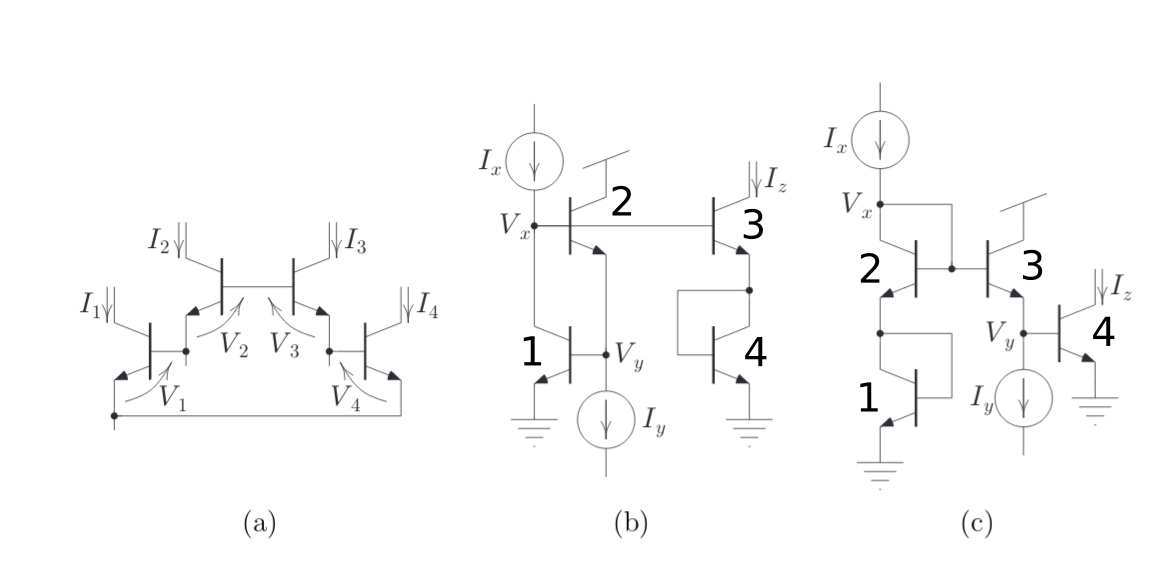
\includegraphics[width=\textwidth]{../circuits1_2.png}
    \caption{}
    \label{fig:1}
\end{figure}

\section{Translinear Circuit 1}
    \begin{itemize}
        \item [(a)]
           All of the transistors will be in forward-active mode. If we first look at transistor 2, we know that it is in forward-active mode because the collector is connected to $V_{cc}$, thus $V_{bc}$ is also reverse biased and $V_{be}$ is forward biased. Since $V_{be}$ for transistor 2 is forward biased, this means that $V_{bc}$ is reverse biased for transistor 1 (since they are connected to the same nets). 

            Transistor 4 is trivially forward-active because it is diode-connected (and thus $V_{bc}$ will always be reverse biased) and the emitter is connected to ground. Transistor 3 due to the problem definition is forward-active.

        \item [(b)]
            Due to the Translinear Principle, $I_z = \sqrt{I_xI_y}$.

        \item [(c)]
            $V_x$ will take a typical value of around twice the turn-on voltage of the transistor ($2 \times 5U_T$), or around $1.2V$. $V_y$ will approximately be the turn-on voltage of the transistor ($5U_T$), $0.6V$.

            We can use the ideal transistor equation to find which input currents the input voltages depend on. $I_x = I_se^{V_y/U_T}$, which can be solved for $V_y$ to find $V_y = U_T\ln\frac{I_x}{I_s}$. Thus, $V_y$ only depends on $I_x$.

            Similarly, $I_y = I_se^{(V_x - V_y)/U_T}$ which we can solve for $V_x$ and find that $V_x = U_T\ln\frac{I_yI_x}{I_s^2}$. Thus, $V_x$ depends on $I_x$ and $I_y$.

    \end{itemize}

\section{Translinear Circuit 2}
    \begin{itemize}
        \item [(a)]
            All of the transistors will be in forward-active mode. Transistor 1 is trivially in forward-active mode because it is diode-connected and has the emitter connected to ground. Transistor 2 is similarly diode-connected, and thus also in forward-active mode.

            Transistor 3 is an emitter-follower and thus will be at least in soft-saturation (which behaves like forward-active mode). From the problem definition, we can assume transistor 4 to be forward-active.

        \item [(b)]
            Due to the Translinear Principle, $I_z = \frac{I_x^2}{I_y}$.

        \item [(c)]
            $V_y$ will take on a value around $5U_T$, or about $0.6V$. $V_x$ is going to be twice the value of $V_y$, approximately, which is about $10U_T$ or $1.2V$.
            
            $V_x$ is completely dependent on $I_x$, since if we assume $\beta$ is infinite, then there is no possible way for another current in the circuit to have an effect on $V_x$. We also know that $I_y = I_se^{(V_x - V_y)/U_T}$, which we can solve for $V_y$ to get $V_y = V_x - U_T\ln\frac{I_y}{I_s}$. This means $V_y$ is dependent on $I_y$ and $I_x$ (since $V_x$ is dependent on $I_x$, and $V_y$ is dependent on $V_x$).

    \end{itemize}

\begin{figure}[h]
    \centering
    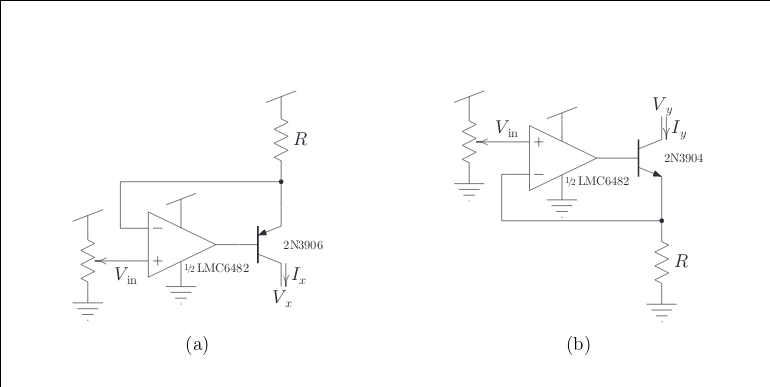
\includegraphics[width=\textwidth]{../circuits2.png}
    \caption{}
    \label{fig:2}
\end{figure}

\section{Current Source/Sink}
    \begin{itemize}
        \item [(a)]
            For circuit (a) the ratio of the potentiometer and R determines the output current. As you increase $V_{in}$, the current, $I_x$, decreases.
            For circuit (b), the ratio of the potentiometer and R determines the output current as well. However, as you increase $V_{in}$, the current, $I_y$, increases.

        \item [(b)]
            For circuit (a) $V_x$ must be a few $U_T$ less than $V_{in}$ because if $V_x$ is greater than $V_{in}$, the transistor will be saturated an will no longer behave like a current source.
            For circuit (b) $V_y$ must be a few $U_T$ greater than $V_{in}$ because if $V_y$ is less than $V_{in}$, the transistor will become saturated and will no longer behave like a current source.
    \end{itemize}

\end{document}
